\documentclass[]{article}
\usepackage{lmodern}
\usepackage{amssymb,amsmath}
\usepackage{ifxetex,ifluatex}
\usepackage{fixltx2e} % provides \textsubscript
\ifnum 0\ifxetex 1\fi\ifluatex 1\fi=0 % if pdftex
  \usepackage[T1]{fontenc}
  \usepackage[utf8]{inputenc}
\else % if luatex or xelatex
  \ifxetex
    \usepackage{mathspec}
  \else
    \usepackage{fontspec}
  \fi
  \defaultfontfeatures{Ligatures=TeX,Scale=MatchLowercase}
\fi
% use upquote if available, for straight quotes in verbatim environments
\IfFileExists{upquote.sty}{\usepackage{upquote}}{}
% use microtype if available
\IfFileExists{microtype.sty}{%
\usepackage{microtype}
\UseMicrotypeSet[protrusion]{basicmath} % disable protrusion for tt fonts
}{}
\usepackage[margin=1in]{geometry}
\usepackage{hyperref}
\hypersetup{unicode=true,
            pdftitle={Course\_Project\_Week2},
            pdfauthor={Chien-Hua Wang},
            pdfborder={0 0 0},
            breaklinks=true}
\urlstyle{same}  % don't use monospace font for urls
\usepackage{color}
\usepackage{fancyvrb}
\newcommand{\VerbBar}{|}
\newcommand{\VERB}{\Verb[commandchars=\\\{\}]}
\DefineVerbatimEnvironment{Highlighting}{Verbatim}{commandchars=\\\{\}}
% Add ',fontsize=\small' for more characters per line
\usepackage{framed}
\definecolor{shadecolor}{RGB}{248,248,248}
\newenvironment{Shaded}{\begin{snugshade}}{\end{snugshade}}
\newcommand{\KeywordTok}[1]{\textcolor[rgb]{0.13,0.29,0.53}{\textbf{#1}}}
\newcommand{\DataTypeTok}[1]{\textcolor[rgb]{0.13,0.29,0.53}{#1}}
\newcommand{\DecValTok}[1]{\textcolor[rgb]{0.00,0.00,0.81}{#1}}
\newcommand{\BaseNTok}[1]{\textcolor[rgb]{0.00,0.00,0.81}{#1}}
\newcommand{\FloatTok}[1]{\textcolor[rgb]{0.00,0.00,0.81}{#1}}
\newcommand{\ConstantTok}[1]{\textcolor[rgb]{0.00,0.00,0.00}{#1}}
\newcommand{\CharTok}[1]{\textcolor[rgb]{0.31,0.60,0.02}{#1}}
\newcommand{\SpecialCharTok}[1]{\textcolor[rgb]{0.00,0.00,0.00}{#1}}
\newcommand{\StringTok}[1]{\textcolor[rgb]{0.31,0.60,0.02}{#1}}
\newcommand{\VerbatimStringTok}[1]{\textcolor[rgb]{0.31,0.60,0.02}{#1}}
\newcommand{\SpecialStringTok}[1]{\textcolor[rgb]{0.31,0.60,0.02}{#1}}
\newcommand{\ImportTok}[1]{#1}
\newcommand{\CommentTok}[1]{\textcolor[rgb]{0.56,0.35,0.01}{\textit{#1}}}
\newcommand{\DocumentationTok}[1]{\textcolor[rgb]{0.56,0.35,0.01}{\textbf{\textit{#1}}}}
\newcommand{\AnnotationTok}[1]{\textcolor[rgb]{0.56,0.35,0.01}{\textbf{\textit{#1}}}}
\newcommand{\CommentVarTok}[1]{\textcolor[rgb]{0.56,0.35,0.01}{\textbf{\textit{#1}}}}
\newcommand{\OtherTok}[1]{\textcolor[rgb]{0.56,0.35,0.01}{#1}}
\newcommand{\FunctionTok}[1]{\textcolor[rgb]{0.00,0.00,0.00}{#1}}
\newcommand{\VariableTok}[1]{\textcolor[rgb]{0.00,0.00,0.00}{#1}}
\newcommand{\ControlFlowTok}[1]{\textcolor[rgb]{0.13,0.29,0.53}{\textbf{#1}}}
\newcommand{\OperatorTok}[1]{\textcolor[rgb]{0.81,0.36,0.00}{\textbf{#1}}}
\newcommand{\BuiltInTok}[1]{#1}
\newcommand{\ExtensionTok}[1]{#1}
\newcommand{\PreprocessorTok}[1]{\textcolor[rgb]{0.56,0.35,0.01}{\textit{#1}}}
\newcommand{\AttributeTok}[1]{\textcolor[rgb]{0.77,0.63,0.00}{#1}}
\newcommand{\RegionMarkerTok}[1]{#1}
\newcommand{\InformationTok}[1]{\textcolor[rgb]{0.56,0.35,0.01}{\textbf{\textit{#1}}}}
\newcommand{\WarningTok}[1]{\textcolor[rgb]{0.56,0.35,0.01}{\textbf{\textit{#1}}}}
\newcommand{\AlertTok}[1]{\textcolor[rgb]{0.94,0.16,0.16}{#1}}
\newcommand{\ErrorTok}[1]{\textcolor[rgb]{0.64,0.00,0.00}{\textbf{#1}}}
\newcommand{\NormalTok}[1]{#1}
\usepackage{graphicx,grffile}
\makeatletter
\def\maxwidth{\ifdim\Gin@nat@width>\linewidth\linewidth\else\Gin@nat@width\fi}
\def\maxheight{\ifdim\Gin@nat@height>\textheight\textheight\else\Gin@nat@height\fi}
\makeatother
% Scale images if necessary, so that they will not overflow the page
% margins by default, and it is still possible to overwrite the defaults
% using explicit options in \includegraphics[width, height, ...]{}
\setkeys{Gin}{width=\maxwidth,height=\maxheight,keepaspectratio}
\IfFileExists{parskip.sty}{%
\usepackage{parskip}
}{% else
\setlength{\parindent}{0pt}
\setlength{\parskip}{6pt plus 2pt minus 1pt}
}
\setlength{\emergencystretch}{3em}  % prevent overfull lines
\providecommand{\tightlist}{%
  \setlength{\itemsep}{0pt}\setlength{\parskip}{0pt}}
\setcounter{secnumdepth}{0}
% Redefines (sub)paragraphs to behave more like sections
\ifx\paragraph\undefined\else
\let\oldparagraph\paragraph
\renewcommand{\paragraph}[1]{\oldparagraph{#1}\mbox{}}
\fi
\ifx\subparagraph\undefined\else
\let\oldsubparagraph\subparagraph
\renewcommand{\subparagraph}[1]{\oldsubparagraph{#1}\mbox{}}
\fi

%%% Use protect on footnotes to avoid problems with footnotes in titles
\let\rmarkdownfootnote\footnote%
\def\footnote{\protect\rmarkdownfootnote}

%%% Change title format to be more compact
\usepackage{titling}

% Create subtitle command for use in maketitle
\newcommand{\subtitle}[1]{
  \posttitle{
    \begin{center}\large#1\end{center}
    }
}

\setlength{\droptitle}{-2em}

  \title{Course\_Project\_Week2}
    \pretitle{\vspace{\droptitle}\centering\huge}
  \posttitle{\par}
    \author{Chien-Hua Wang}
    \preauthor{\centering\large\emph}
  \postauthor{\par}
      \predate{\centering\large\emph}
  \postdate{\par}
    \date{January 16, 2019}


\begin{document}
\maketitle

\subsection{download zip file containing data if it hasn't already been
downloaded}\label{download-zip-file-containing-data-if-it-hasnt-already-been-downloaded}

\begin{Shaded}
\begin{Highlighting}[]
\NormalTok{zipUrl <-}\StringTok{ "https://d396qusza40orc.cloudfront.net/repdata%2Fdata%2Factivity.zip"}
\NormalTok{zipFile <-}\StringTok{ "Activity Monitoring Data.zip"}
\ControlFlowTok{if}\NormalTok{ (}\OperatorTok{!}\KeywordTok{file.exists}\NormalTok{(zipFile)) \{}
  \KeywordTok{download.file}\NormalTok{(zipUrl, zipFile, }\DataTypeTok{mode =} \StringTok{"wb"}\NormalTok{)}
\NormalTok{\}}
\end{Highlighting}
\end{Shaded}

\subsection{unzip zip file containing data if data directory doesn't
already
exist}\label{unzip-zip-file-containing-data-if-data-directory-doesnt-already-exist}

\begin{Shaded}
\begin{Highlighting}[]
\NormalTok{dataPath <-}\StringTok{ "Activity Monitoring Data"}
\ControlFlowTok{if}\NormalTok{ (}\OperatorTok{!}\KeywordTok{file.exists}\NormalTok{(dataPath)) \{}
  \KeywordTok{unzip}\NormalTok{(zipFile)}
\NormalTok{\}}
\end{Highlighting}
\end{Shaded}

\subsection{Import data}\label{import-data}

\begin{Shaded}
\begin{Highlighting}[]
\NormalTok{activitydf <-}\StringTok{ }\KeywordTok{read.csv}\NormalTok{(}\StringTok{"activity.csv"}\NormalTok{)}
\CommentTok{# Format steps and date }
\NormalTok{activitydf}\OperatorTok{$}\NormalTok{date =}\StringTok{ }\KeywordTok{as.Date}\NormalTok{(activitydf}\OperatorTok{$}\NormalTok{date)}
\end{Highlighting}
\end{Shaded}

\subsubsection{1. Calculate the total number of steps taken per
day}\label{calculate-the-total-number-of-steps-taken-per-day}

\begin{Shaded}
\begin{Highlighting}[]
\NormalTok{Total_Steps =}\StringTok{ }\NormalTok{activitydf }\OperatorTok
\StringTok{  }\KeywordTok{select}\NormalTok{(date, steps) }\OperatorTok
\StringTok{  }\KeywordTok{group_by}\NormalTok{(date) }\OperatorTok
\StringTok{  }\KeywordTok{summarize}\NormalTok{(}\DataTypeTok{steps =} \KeywordTok{sum}\NormalTok{(steps))}
\KeywordTok{head}\NormalTok{(Total_Steps,}\DecValTok{10}\NormalTok{)}
\end{Highlighting}
\end{Shaded}

\begin{verbatim}
## # A tibble: 10 x 2
##    date       steps
##    <date>     <int>
##  1 2012-10-01    NA
##  2 2012-10-02   126
##  3 2012-10-03 11352
##  4 2012-10-04 12116
##  5 2012-10-05 13294
##  6 2012-10-06 15420
##  7 2012-10-07 11015
##  8 2012-10-08    NA
##  9 2012-10-09 12811
## 10 2012-10-10  9900
\end{verbatim}

\subsubsection{2. Histogram of the total number of steps taken each
day}\label{histogram-of-the-total-number-of-steps-taken-each-day}

\begin{Shaded}
\begin{Highlighting}[]
\KeywordTok{ggplot}\NormalTok{(Total_Steps, }\KeywordTok{aes}\NormalTok{(}\DataTypeTok{x =}\NormalTok{ steps)) }\OperatorTok{+}
\StringTok{  }\KeywordTok{geom_histogram}\NormalTok{(}\DataTypeTok{fill =} \StringTok{"blue"}\NormalTok{, }\DataTypeTok{binwidth =} \DecValTok{900}\NormalTok{) }\OperatorTok{+}
\StringTok{  }\KeywordTok{labs}\NormalTok{(}\DataTypeTok{title =} \StringTok{"Daily Steps"}\NormalTok{, }\DataTypeTok{x =} \StringTok{"Steps"}\NormalTok{, }\DataTypeTok{y =} \StringTok{"Frequency"}\NormalTok{)}
\end{Highlighting}
\end{Shaded}

\begin{verbatim}
## Warning: Removed 8 rows containing non-finite values (stat_bin).
\end{verbatim}

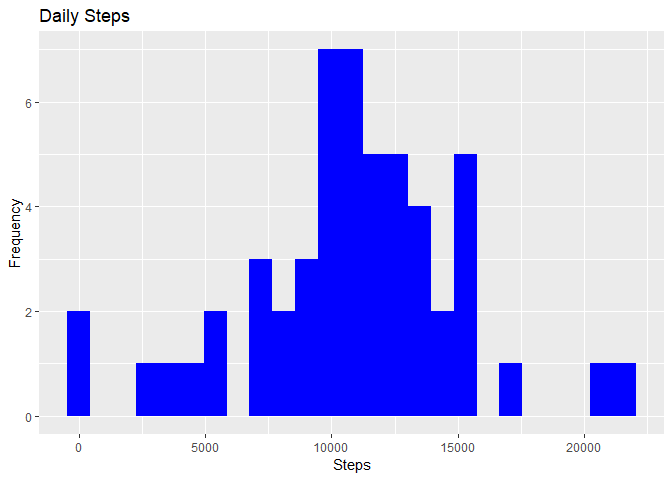
\includegraphics{PA1_template_files/figure-latex/unnamed-chunk-5-1.pdf}

\subsubsection{3. Mean and median number of steps taken each
day}\label{mean-and-median-number-of-steps-taken-each-day}

\begin{Shaded}
\begin{Highlighting}[]
\NormalTok{Total_Steps }\OperatorTok
\StringTok{  }\KeywordTok{select}\NormalTok{(steps) }\OperatorTok
\StringTok{  }\KeywordTok{summarise}\NormalTok{(}\DataTypeTok{Mean_Steps =} \KeywordTok{mean}\NormalTok{(steps,}\DataTypeTok{na.rm=}\NormalTok{T),}
            \DataTypeTok{Media_Steps =} \KeywordTok{median}\NormalTok{(steps, }\DataTypeTok{na.rm=}\NormalTok{T))}
\end{Highlighting}
\end{Shaded}

\begin{verbatim}
## # A tibble: 1 x 2
##   Mean_Steps Media_Steps
##        <dbl>       <int>
## 1     10766.       10765
\end{verbatim}

\subsubsection{4. Time series plot of the average number of steps
taken}\label{time-series-plot-of-the-average-number-of-steps-taken}

\begin{Shaded}
\begin{Highlighting}[]
\NormalTok{Intervaldf =}\StringTok{ }\NormalTok{activitydf }\OperatorTok
\StringTok{  }\KeywordTok{select}\NormalTok{(steps, interval) }\OperatorTok
\StringTok{  }\KeywordTok{group_by}\NormalTok{(interval) }\OperatorTok
\StringTok{  }\KeywordTok{summarise}\NormalTok{(}\DataTypeTok{steps =} \KeywordTok{mean}\NormalTok{(steps, }\DataTypeTok{na.rm=}\NormalTok{T))}
\KeywordTok{ggplot}\NormalTok{(Intervaldf, }\KeywordTok{aes}\NormalTok{(}\DataTypeTok{x =}\NormalTok{ interval , }\DataTypeTok{y =}\NormalTok{ steps)) }\OperatorTok{+}\StringTok{ }\KeywordTok{geom_line}\NormalTok{(}\DataTypeTok{color=}\StringTok{"blue"}\NormalTok{, }\DataTypeTok{size=}\DecValTok{1}\NormalTok{) }\OperatorTok{+}\StringTok{ }\KeywordTok{labs}\NormalTok{(}\DataTypeTok{title =} \StringTok{"Avg. Daily Steps"}\NormalTok{, }\DataTypeTok{x =} \StringTok{"Interval"}\NormalTok{, }\DataTypeTok{y =} \StringTok{"Avg. Steps per day"}\NormalTok{)}
\end{Highlighting}
\end{Shaded}

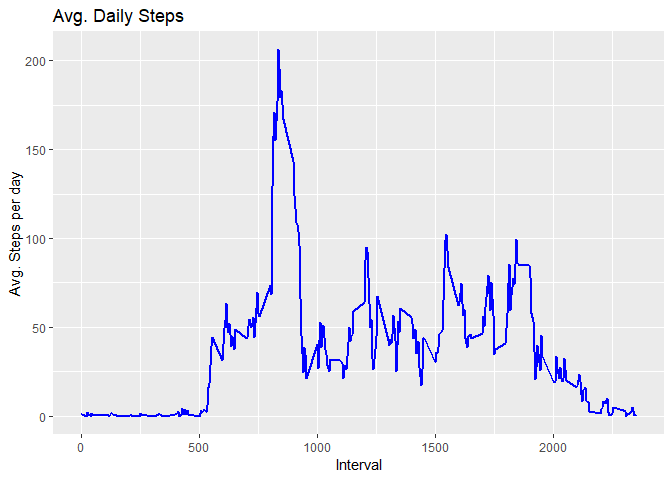
\includegraphics{PA1_template_files/figure-latex/unnamed-chunk-7-1.pdf}

\subsubsection{5. The 5-minute interval that, on average, contains the
maximum number of
steps}\label{the-5-minute-interval-that-on-average-contains-the-maximum-number-of-steps}

\begin{Shaded}
\begin{Highlighting}[]
\NormalTok{Intervaldf }\OperatorTok
\StringTok{  }\KeywordTok{filter}\NormalTok{(steps }\OperatorTok{==}\StringTok{ }\KeywordTok{max}\NormalTok{(steps)) }\OperatorTok
\StringTok{  }\KeywordTok{select}\NormalTok{(interval) }\OperatorTok
\StringTok{  }\KeywordTok{summarize}\NormalTok{(}\DataTypeTok{max_interval =}\NormalTok{ interval)}
\end{Highlighting}
\end{Shaded}

\begin{verbatim}
## # A tibble: 1 x 1
##   max_interval
##          <int>
## 1          835
\end{verbatim}

\subsubsection{6. Code to describe and show a strategy for imputing
missing
data}\label{code-to-describe-and-show-a-strategy-for-imputing-missing-data}

\paragraph{Using the mean value to fill
NA}\label{using-the-mean-value-to-fill-na}

\begin{Shaded}
\begin{Highlighting}[]
\KeywordTok{sapply}\NormalTok{(activitydf,}\ControlFlowTok{function}\NormalTok{(x) }\KeywordTok{sum}\NormalTok{(}\KeywordTok{is.na}\NormalTok{(x)))}
\end{Highlighting}
\end{Shaded}

\begin{verbatim}
##    steps     date interval 
##     2304        0        0
\end{verbatim}

\begin{Shaded}
\begin{Highlighting}[]
\NormalTok{newactivitydf =}\StringTok{ }\NormalTok{activitydf }\OperatorTok
\StringTok{  }\KeywordTok{mutate}\NormalTok{(}\DataTypeTok{steps =} \KeywordTok{replace_na}\NormalTok{(steps,}\KeywordTok{mean}\NormalTok{(steps,}\DataTypeTok{na.rm=}\NormalTok{T)))}

\KeywordTok{sapply}\NormalTok{(newactivitydf,}\ControlFlowTok{function}\NormalTok{(x) }\KeywordTok{sum}\NormalTok{(}\KeywordTok{is.na}\NormalTok{(x)))}
\end{Highlighting}
\end{Shaded}

\begin{verbatim}
##    steps     date interval 
##        0        0        0
\end{verbatim}

\begin{Shaded}
\begin{Highlighting}[]
\CommentTok{# Create a new dataset that is equal to the original dataset but with the missing data filled in.}
\CommentTok{# write.csv(newactivitydf,file='tidyData_activity.csv')}
\end{Highlighting}
\end{Shaded}

\subsubsection{7. Histogram of the total number of steps taken each day
after missing values are
imputed}\label{histogram-of-the-total-number-of-steps-taken-each-day-after-missing-values-are-imputed}

\begin{Shaded}
\begin{Highlighting}[]
\NormalTok{Total_Steps =}\StringTok{ }\NormalTok{newactivitydf }\OperatorTok
\StringTok{  }\KeywordTok{select}\NormalTok{(date, steps) }\OperatorTok
\StringTok{  }\KeywordTok{group_by}\NormalTok{(date) }\OperatorTok
\StringTok{  }\KeywordTok{summarize}\NormalTok{(}\DataTypeTok{steps =} \KeywordTok{sum}\NormalTok{(steps))}

\KeywordTok{ggplot}\NormalTok{(Total_Steps, }\KeywordTok{aes}\NormalTok{(}\DataTypeTok{x =}\NormalTok{ steps)) }\OperatorTok{+}
\StringTok{  }\KeywordTok{geom_histogram}\NormalTok{(}\DataTypeTok{fill =} \StringTok{"blue"}\NormalTok{, }\DataTypeTok{binwidth =} \DecValTok{900}\NormalTok{) }\OperatorTok{+}
\StringTok{  }\KeywordTok{labs}\NormalTok{(}\DataTypeTok{title =} \StringTok{"Daily Steps"}\NormalTok{, }\DataTypeTok{x =} \StringTok{"Steps"}\NormalTok{, }\DataTypeTok{y =} \StringTok{"Frequency"}\NormalTok{)}
\end{Highlighting}
\end{Shaded}

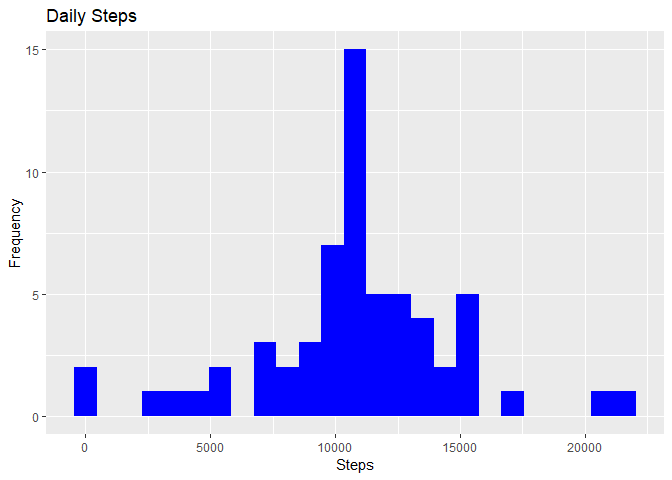
\includegraphics{PA1_template_files/figure-latex/unnamed-chunk-10-1.pdf}

\begin{Shaded}
\begin{Highlighting}[]
\NormalTok{Total_Steps }\OperatorTok
\StringTok{  }\KeywordTok{select}\NormalTok{(steps) }\OperatorTok
\StringTok{  }\KeywordTok{summarise}\NormalTok{(}\DataTypeTok{Mean_Steps =} \KeywordTok{mean}\NormalTok{(steps,}\DataTypeTok{na.rm=}\NormalTok{T),}
            \DataTypeTok{Media_Steps =} \KeywordTok{median}\NormalTok{(steps, }\DataTypeTok{na.rm=}\NormalTok{T))}
\end{Highlighting}
\end{Shaded}

\begin{verbatim}
## # A tibble: 1 x 2
##   Mean_Steps Media_Steps
##        <dbl>       <dbl>
## 1     10766.      10766.
\end{verbatim}

\subsubsection{8.Panel plot comparing the average number of steps taken
per 5-minute interval across weekdays and
weekends}\label{panel-plot-comparing-the-average-number-of-steps-taken-per-5-minute-interval-across-weekdays-and-weekends}

\begin{Shaded}
\begin{Highlighting}[]
\NormalTok{activitydf <-}\StringTok{ }\KeywordTok{read.csv}\NormalTok{(}\StringTok{"activity.csv"}\NormalTok{)}
\NormalTok{activitydf =}\StringTok{ }\NormalTok{activitydf }\OperatorTok
\StringTok{  }\KeywordTok{mutate}\NormalTok{(}\DataTypeTok{steps =} \KeywordTok{replace_na}\NormalTok{(steps,}\KeywordTok{mean}\NormalTok{(steps,}\DataTypeTok{na.rm=}\NormalTok{T)),}
         \DataTypeTok{date =} \KeywordTok{as.Date}\NormalTok{(date),}
         \StringTok{`}\DataTypeTok{Day of week}\StringTok{`}\NormalTok{ =}\StringTok{ }\KeywordTok{weekdays}\NormalTok{(date),}
         \StringTok{`}\DataTypeTok{weekday or weekend}\StringTok{`}\NormalTok{ =}\StringTok{ }\KeywordTok{ifelse}\NormalTok{(}\KeywordTok{grepl}\NormalTok{(}\DataTypeTok{pattern =} \StringTok{"Monday|Tuesday|Wednesday|Thursday|Friday"}\NormalTok{,}\StringTok{`}\DataTypeTok{Day of week}\StringTok{`}\NormalTok{),}\StringTok{"weekday"}\NormalTok{, }\StringTok{"weekend"}\NormalTok{),}
         \StringTok{`}\DataTypeTok{weekday or weekend}\StringTok{`}\NormalTok{ =}\StringTok{ }\KeywordTok{as.factor}\NormalTok{(}\StringTok{`}\DataTypeTok{weekday or weekend}\StringTok{`}\NormalTok{)) }\OperatorTok
\StringTok{  }\KeywordTok{select}\NormalTok{(}\KeywordTok{everything}\NormalTok{()) }\OperatorTok
\StringTok{  }\KeywordTok{group_by}\NormalTok{(interval, }\StringTok{`}\DataTypeTok{weekday or weekend}\StringTok{`}\NormalTok{) }\OperatorTok
\StringTok{  }\KeywordTok{summarise}\NormalTok{(}\DataTypeTok{steps =} \KeywordTok{mean}\NormalTok{(steps))}

\KeywordTok{ggplot}\NormalTok{(activitydf , }\KeywordTok{aes}\NormalTok{(}\DataTypeTok{x =}\NormalTok{ interval , }\DataTypeTok{y =}\NormalTok{ steps, }\DataTypeTok{color=}\StringTok{`}\DataTypeTok{weekday or weekend}\StringTok{`}\NormalTok{)) }\OperatorTok{+}\StringTok{ }\KeywordTok{geom_line}\NormalTok{() }\OperatorTok{+}\StringTok{ }\KeywordTok{labs}\NormalTok{(}\DataTypeTok{title =} \StringTok{"Avg. Daily Steps by Weektype"}\NormalTok{, }\DataTypeTok{x =} \StringTok{"Interval"}\NormalTok{, }\DataTypeTok{y =} \StringTok{"No. of Steps"}\NormalTok{) }\OperatorTok{+}\StringTok{ }\KeywordTok{facet_wrap}\NormalTok{(}\OperatorTok{~}\StringTok{`}\DataTypeTok{weekday or weekend}\StringTok{`}\NormalTok{ , }\DataTypeTok{ncol =} \DecValTok{1}\NormalTok{, }\DataTypeTok{nrow=}\DecValTok{2}\NormalTok{)}
\end{Highlighting}
\end{Shaded}

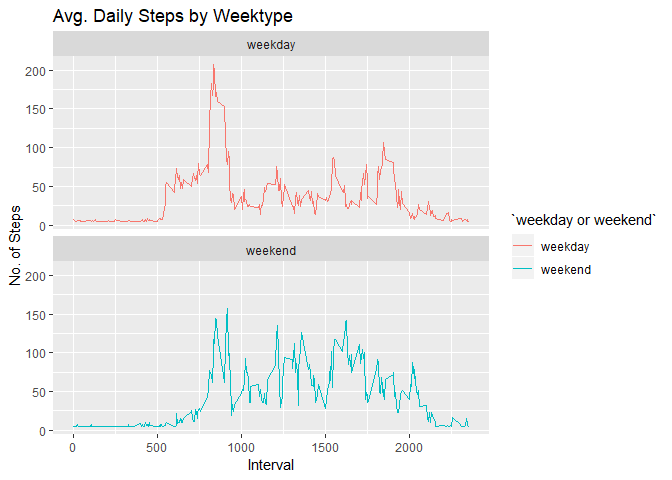
\includegraphics{PA1_template_files/figure-latex/unnamed-chunk-11-1.pdf}


\end{document}
